 \documentclass[12pt,a4paper]{article}

% Essential packages
\usepackage[utf8]{inputenc}
\usepackage[T1]{fontenc}
\usepackage{graphicx}
\usepackage{amsmath}
\usepackage{booktabs}
\usepackage[table]{xcolor}
\usepackage{float}
\usepackage{hyperref}
\usepackage{siunitx}
\usepackage{caption}
\usepackage{subcaption}
\usepackage[margin=2.5cm]{geometry}

% Custom colors for tables and figures
\definecolor{lightgray}{gray}{0.95}
\definecolor{mediumgray}{gray}{0.85}

% Title information

\usepackage{authblk} % For author and affiliation

% Title information
\title{\textbf{Dynamic Epidemic Propagation in Community-Structured Networks}}

% Author information
\author{Arjun K. Nandan} % Corrected formatting
\affil{Department of Humanities and Social Sciences, Indian Institute of Technology, Roorkee \\ 
\texttt{arjun\_kn@hs.iitr.ac.in}} % Corrected email formatting

% Include today's date
\date{\today} 






\begin{document}

\maketitle

\begin{abstract}
This study investigates the dynamics of epidemic spread across networks with varying community structures using Stochastic Block Models (SBM) and modified SIR (Susceptible-Infected-Recovered) dynamics. We analyze three distinct network configurations—sparse, balanced, and dense inter-community connections—each comprising two communities of 50 nodes. By incorporating a dynamic transmission rate that responds to population states, we demonstrate how network topology influences epidemic progression. Our findings reveal that while denser inter-community connections accelerate infection peaks and reduce time to maximum spread, the final outbreak size remains relatively consistent across configurations. These results provide insights into the relationship between community structure and disease propagation, with implications for public health interventions.
\end{abstract}


\section{Introduction}
The study of epidemic spread through structured populations has become increasingly crucial for understanding and managing disease outbreaks in our interconnected world. Network theory provides a powerful framework for modeling these complex interactions, particularly when considering how community structures influence disease transmission dynamics. This research employs Stochastic Block Models (SBM) to investigate how varying degrees of inter-community connectivity affect epidemic propagation patterns. By examining three distinct network configurations—spanning from highly segregated to well-connected communities—we explore the interplay between network topology and disease spread. Our approach incorporates a dynamic SIR model with an adaptive transmission rate that responds to both the current infection state and recovered population, reflecting real-world behavioral changes and immunity effects. This methodology enables us to capture both the structural aspects of social networks and the temporal evolution of disease spread, providing a comprehensive framework for understanding how community structures influence epidemic dynamics.


\section{Methodology}


\subsection{Network Structures}




The Stochastic Block Model (SBM) was chosen as the basis for this analysis due to its inherent ability to model networks with well-defined community structures. Unlike other random graph models, SBM allows for the specification of connection probabilities within and between communities, making it highly effective for simulating realistic social networks where interactions vary significantly between groups. This feature is crucial for studying the dynamics of phenomena such as epidemic spread, where community structure plays a pivotal role in determining how quickly and widely an infection propagates. The SBM’s flexibility in adjusting intra- and inter-community connection probabilities provides a way to capture different network topologies, ranging from highly segregated to highly interconnected communities. This adaptability is key to analyzing and comparing various scenarios that represent different levels of social cohesion and interaction.

\begin{figure}[H]
    \centering
    \includegraphics[width=1\linewidth]{stochastic_block_models.png}
    \caption{Stochastic Block Model Configurations}
    \label{fig:enter-label}
\end{figure}

In this analysis, three SBM configurations were chosen to reflect networks with varying degrees of connectivity between two communities of 50 nodes each. The \textbf{Sparse Inter-Community Network} is defined by an intra-community connection probability of 0.1 and a minimal inter-community probability of 0.001. This network structure models a scenario where communities are tightly knit internally but have minimal interactions with each other. Such a setup helps study epidemic dynamics within isolated groups and the delayed transmission between them, highlighting how community boundaries can act as barriers to disease spread. In contrast, the \textbf{Balanced Network} increases the inter-community connection probability to 0.01 while maintaining the intra-community probability of 0.1. This configuration represents a network where communities have moderate interaction, allowing for analysis of scenarios where the epidemic can spread beyond the confines of a single community but still faces some resistance at the community boundary.

Finally, the \textbf{Dense Inter-Community Network} features an inter-community probability of 0.05, while keeping the intra-community connection at 0.1. This configuration simulates a network where communities are sufficiently interconnected to reduce the distinction between them. Such a structure is ideal for observing rapid epidemic spread due to shorter paths and greater connectivity, leading to almost immediate cross-community transmission.

The SBM adjacency matrices are configured as:
\[
\mathbf{P} =
\begin{bmatrix}
0.1 & p \\
p & 0.1
\end{bmatrix},
\]
where \(p \in \{0.001, 0.01, 0.05\}\) represents different levels of inter-community connection probabilities.

Choosing SBM for this analysis is reasoned by its capacity to realistically mimic social structures where clustering within groups and the strength of inter-group connections can dramatically alter the trajectory of an epidemic. Studying networks that range from isolated clusters to highly interconnected systems provides valuable insights into how structural properties like density, clustering, and average path length influence the spread of an infection. This, in turn, aids in designing more effective strategies for controlling outbreaks by understanding which network features accelerate or impede disease transmission.





\subsection{Epidemic Model and Parameters}

In this study, we use a dynamic SIR (Susceptible-Infected-Recovered) model to simulate the spread of an epidemic over stochastic block model (SBM) networks. The SBM configuration represents distinct communities with varying inter-community connection probabilities. The SIR model is defined as follows:

\subsubsection*{SIR Model Equations}
The SIR model describes the dynamics of an epidemic through the following differential equations:

\begin{align}
    \frac{dS(t)}{dt} &= -\tau(t) S(t) I(t), \\
    \frac{dI(t)}{dt} &= \tau(t) S(t) I(t) - \gamma I(t), \\
    \frac{dR(t)}{dt} &= \gamma I(t),
\end{align}

where:
\begin{itemize}
    \item \(S(t)\): Number of susceptible individuals at time \(t\). These are individuals who have not yet been infected but are at risk.
    \item \(I(t)\): Number of infected individuals at time \(t\). These are individuals currently capable of spreading the disease.
    \item \(R(t)\): Number of recovered individuals at time \(t\). These individuals have recovered and gained immunity, thus no longer participating in disease transmission.
    \item \(\tau(t)\): Dynamic transmission rate, representing the rate at which susceptible individuals become infected, which varies over time.
    \item \(\gamma\): Recovery rate, representing the rate at which infected individuals recover and move to the recovered state. A constant value is assumed in this study.
\end{itemize}

\subsubsection*{Dynamic Transmission Rate \(\tau(t)\)}
The transmission rate \(\tau(t)\) is modeled as a dynamic parameter that adapts to the current state of the epidemic. It is defined as:

\begin{equation}
    \tau(t) = \max\left(0.1 \cdot \tau_0, \tau_0 \cdot (1 - I_f(t)) \cdot (1 - 0.5 \cdot R_f(t))\right),
\end{equation}

where:
\begin{itemize}
    \item \(\tau_0\): Base transmission rate, representing the transmission rate in the absence of any behavioral changes or immunity effects.
    \item \(I_f(t) = \frac{I(t)}{N}\): Fraction of the population currently infected. As this increases, \(\tau(t)\) decreases, reflecting behavioral changes like increased social distancing or precautionary measures.
    \item \(R_f(t) = \frac{R(t)}{N}\): Fraction of the population recovered. This contributes to herd immunity, reducing the effective transmission rate.
    \item \(N\): Total population size.
\end{itemize}

\subsubsection*{}
The dynamic \(\tau(t)\) is designed to capture two critical real-world phenomena:
\begin{enumerate}
    \item \textbf{Behavioral Response:} 
    As the number of infected individuals increases, individuals in the population are likely to adopt more cautious behavior, such as social distancing or wearing masks. This behavioral shift reduces the effective contact rate, thereby lowering the transmission rate.
    
    \item \textbf{Immunity Effect:} 
    The recovered population contributes to herd immunity. As more individuals recover, the pool of susceptible individuals shrinks, reducing the likelihood of disease transmission. In this model, the recovered population reduces the transmission rate by up to 50\%, reflecting their immunity's protective effect on the overall community.
    
    \item \textbf{Safeguard Mechanism:} 
    To prevent the transmission rate from dropping unrealistically low, a minimum transmission rate of \(0.1 \cdot \tau_0\) is imposed. This ensures that the disease spread does not halt entirely due to stochastic noise, maintaining model stability.
\end{enumerate}


\subsubsection*{Simulation Parameters}
The key parameters used in the simulation are:
\begin{itemize}
    \item \(N = 100\): Total population size.
    \item \textbf{Initial number of infected individuals:} 1 individual is initially infected.
    \item \(\gamma = 0.1\): Recovery rate. This parameter determines the average time an individual remains infected.
    \item \(\tau_0 = 0.3\): Base transmission rate. This serves as the starting point for calculating \(\tau(t)\).
    \item \textbf{Simulation time steps:} 100, ensuring sufficient time for observing the epidemic's progression.
\end{itemize}
















\section{Results}
\subsection{Network Characteristics}
\begin{table}[H]
\centering
\caption{Network Topology Metrics}
\begin{tabular}{lccc}
\toprule
\textbf{Metric} & \textbf{Sparse Inter} & \textbf{Balanced} & \textbf{Dense Inter} \\
\midrule
Average Degree & 5.32 & 5.88 & 7.76 \\
Average Path Length & 3.73 & 2.98 & 2.45 \\
Network Diameter & 9 & 6 & 4 \\
Assortativity (Degree Correlation) & 0.012 & -0.009 & 0.008 \\
Number of Communities (Approx.) & 2 & 2 & 2 \\
\bottomrule
\end{tabular}
\label{tab:network_topology_metrics}
\end{table}
Table \ref{tab:network_topology_metrics} outlines the core topology metrics for Sparse, Balanced, and Dense network configurations. The \textbf{Average Degree} indicates that Dense Inter networks have the highest connectivity per node at 7.76, followed by the Balanced network at 5.88 and Sparse Inter at 5.32, suggesting greater potential for information or contagion spread within the Dense Inter network.The \textbf{Average Path Length} decreases as connectivity increases, with Dense Inter networks demonstrating the shortest path length of 2.45, indicating faster reachability within the network. Conversely, the Sparse Inter network, with an average path length of 3.73, requires more steps for information to propagate, aligning with its lower connectivity.The \textbf{Network Diameter} values further support this observation, with Dense Inter at 4 and Sparse Inter at 9, indicating a wider spread of distances in the latter.The \textbf{Assortativity} values, ranging from weakly positive (Sparse Inter and Dense Inter) to weakly negative (Balanced), suggest minimal preference for nodes to connect with others of similar degree. All three network types have an approximate community structure of two, emphasizing similar modularity across configurations.



\subsection{Epidemic Dynamics}

Figure~\ref{fig:epidemic_curves} consists of six panels arranged in a 3 × 2 grid, corresponding to three network configurations: Sparse, Balanced, and Dense Inter-Community Networks. Each row represents a different network type, with the left panel depicting the epidemic curves (Susceptible, Infected, and Recovered populations) over time, and the right panel showing the dynamic transmission rate (\(\tau\)) as it evolves during the simulation.
\begin{figure}[H]
    \centering
    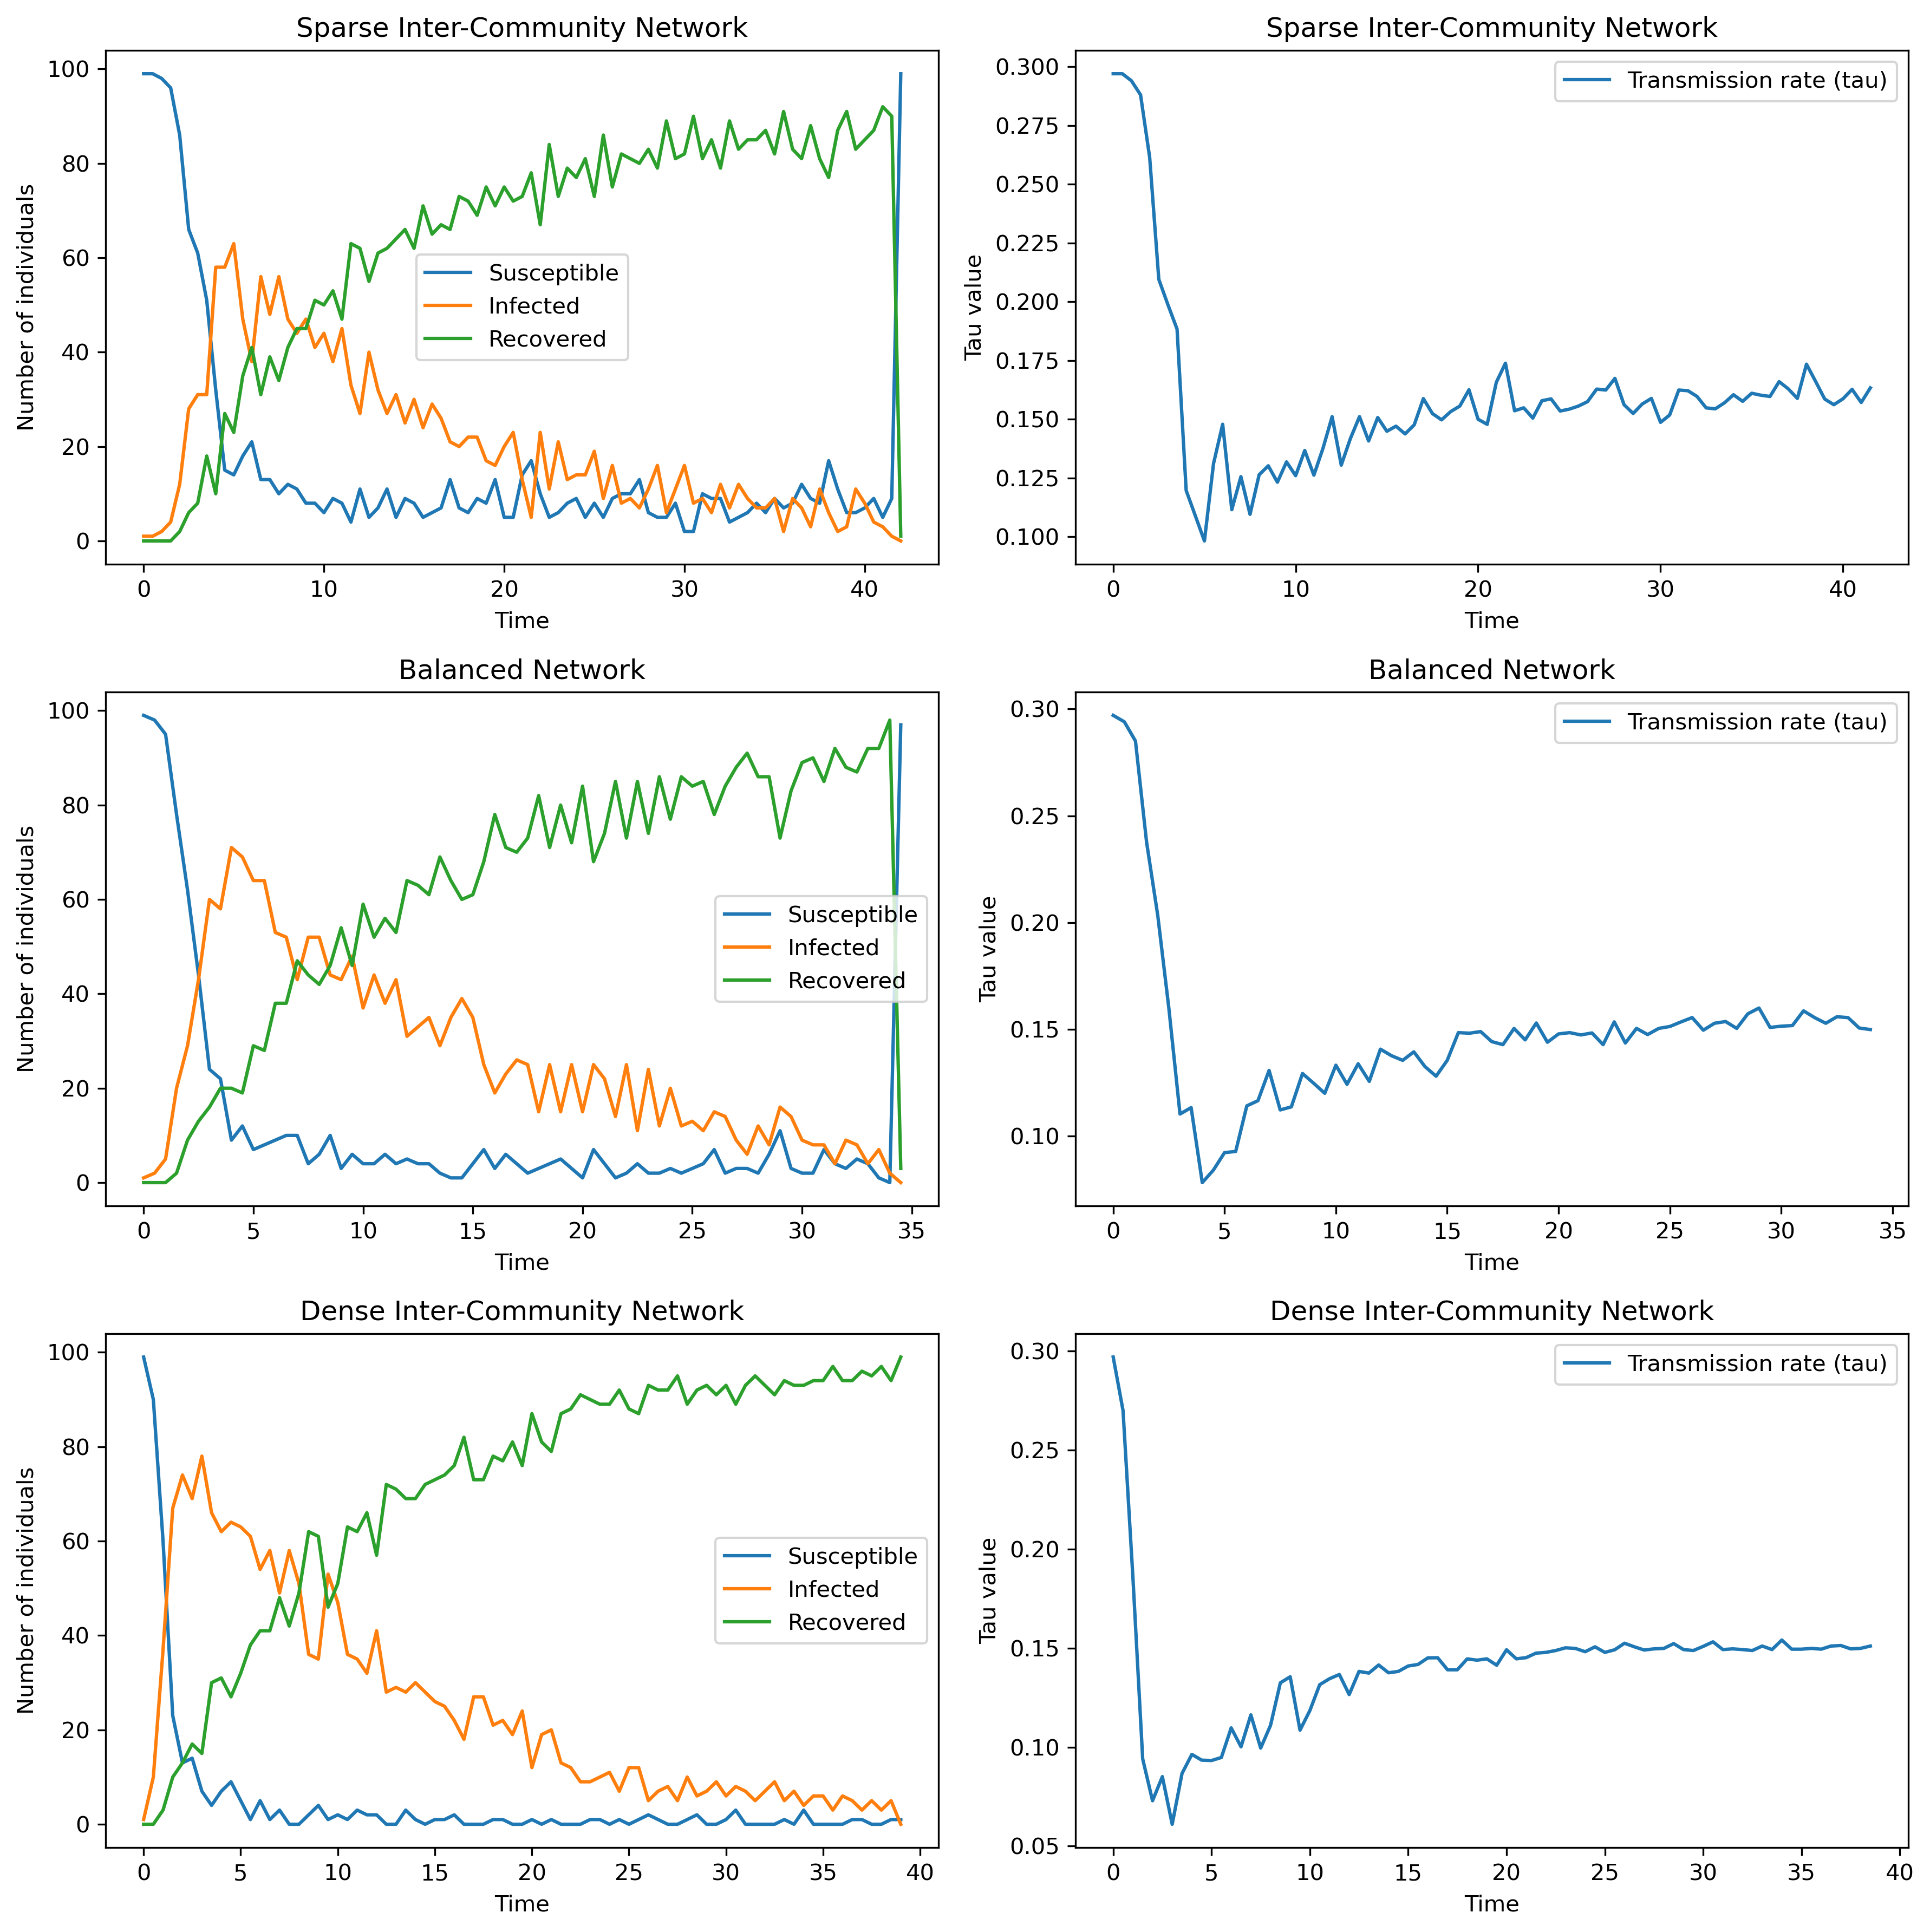
\includegraphics[width=1\linewidth]{Epidemics.png}
    \caption{Comparison of Infection Curves Across Network Types}
    \label{fig:epidemic_curves}
\end{figure}
In the left panels, the horizontal axis represents time, while the vertical axis indicates the number of individuals in each epidemiological state. These curves illustrate how infection spreads differently based on the underlying network structure. In the right panels, the horizontal axis is again time, while the vertical axis shows the corresponding transmission rate (\(\tau\)), which adjusts dynamically based on network and epidemic states. This allows for a detailed comparison of how transmission potential changes across varying network configurations.

The panels collectively provide insights into the interplay between network structure and epidemic dynamics, highlighting the differences in infection peaks and recovery trends. This visualization serves as a foundation for analyzing the spread of infection and the influence of dynamic transmission rates under different connectivity scenarios, as detailed in the subsequent analysis.



\subsection{Peak Infection Analysis}
\begin{table}[H]
\centering
\caption{Peak Infection Metrics Across Network Types}
\begin{tabular}{lccc}
\toprule
\textbf{Metric} & \textbf{Sparse Inter} & \textbf{Balanced} & \textbf{Dense Inter} \\
\midrule
\multicolumn{4}{c}{\textbf{Peak Infection Metrics}} \\
\midrule
Mean Peak (\%)   & 58.523 & 62.341 & 69.967 \\
Std. Dev Peak    & 18.318 & 19.335 & 16.764 \\
Median Peak (\%) & 64.0   & 68.0   & 74.0   \\
\midrule
\multicolumn{4}{c}{\textbf{Time to Peak (Time Steps)}} \\
\midrule
Mean Time        & 3.8995 & 3.1190 & 2.4945 \\
Std. Dev Time    & 1.5549 & 1.2520 & 0.8983 \\
Median Time      & 4.0    & 3.0    & 2.5    \\
\midrule
\multicolumn{4}{c}{\textbf{Outbreak Size Metrics (\% Population Infected)}} \\
\midrule
Mean Outbreak    & 38.664 & 39.073 & 38.870 \\
Std. Dev Outbreak & 12.552 & 12.472 & 9.886 \\
Median Outbreak  & 42.0   & 42.5   & 41.0   \\
\bottomrule
\end{tabular}
\label{tab:peak_metrics}
\end{table}

Table \ref{tab:peak_metrics} provides a comparative overview of infection dynamics across three network structures: Sparse, Balanced, and Dense. The analysis captures distinctions in peak infection rates, the time required to reach peak infection, and the overall outbreak size as a percentage of the population. Under the \textbf{Peak Infection Metrics} category, the Dense network exhibits the highest mean peak infection rate at 69.97\%, with a median of 74\%. This result indicates that higher interconnectedness facilitates a more extensive spread, likely due to the greater frequency of inter-community connections. In contrast, the Sparse network achieves a lower mean peak infection rate of 58.52\%, suggesting a reduced capacity for rapid infection spread across the network, reflective of its limited connectivity.

The \textbf{Time to Peak} metrics further underscore these differences. Dense networks, with a mean time to peak of 2.49 time steps and a relatively low standard deviation, demonstrate rapid and consistent transmission patterns, indicative of robust inter-community links enabling swift contagion spread. Conversely, the Sparse network requires an average of 3.90 time steps to reach peak infection, consistent with its more isolated structure that impedes quick transmission.

The \textbf{Outbreak Size Metrics} indicate that all networks ultimately infect a similar portion of the population, averaging around 38-39\%. This outcome suggests that while network density significantly influences the rate and timing of peak infections, it does not drastically affect the total outbreak size, which remains comparable across network types.


\subsection{Community Impact Analysis}
The analysis of epidemic spread across different network topologies underscores the significant role of community structure in shaping disease transmission dynamics. In the \textbf{Sparse Inter-Community Network}, characterized by limited inter-community connections, the infection spreads slowly, with a delayed peak in the number of infected individuals. The gradual decline in the susceptible population and steady increase in recoveries indicate that the network's low connectivity acts as a barrier to rapid transmission. This is further corroborated by the dynamic transmission rate (\(\tau\)), which starts high but declines sharply and stabilizes at a low value, reflecting limited opportunities for cross-community infections (see Figure~\ref{fig:epidemic_curves}).

In contrast, the \textbf{Balanced Network}, with moderate inter-community connections, facilitates a faster spread of infection compared to the sparse configuration. The infection curve peaks earlier, and the recovery phase progresses more quickly, highlighting the network's increased ability to transmit the disease beyond individual communities. The dynamic \(\tau\) in this network shows a decline from its initial value but stabilizes at a moderate level, reflecting sustained transmission potential due to balanced interconnectivity. This network configuration models scenarios where moderate social interactions exist, leading to a more synchronized spread across communities.

The \textbf{Dense Inter-Community Network} presents a scenario of high interconnectivity, where the infection spreads rapidly, peaking early and resulting in a swift decline in the susceptible population. This configuration demonstrates how high connectivity facilitates widespread and accelerated transmission, as evidenced by the epidemic curve and a relatively high stabilized \(\tau\). The dense network provides critical insights into scenarios of high social cohesion, where community boundaries blur, leading to near-simultaneous outbreaks across the network. These findings collectively emphasize the importance of network structure and dynamic transmission rates in understanding and managing epidemic spread effectively.



\section{Conclusion}
This study demonstrates the significant influence of network topology on epidemic propagation, particularly highlighting how inter-community connection patterns shape disease transmission dynamics. Our analysis of three distinct network configurations—sparse, balanced, and dense—reveals that while higher connectivity accelerates infection peaks and reduces time to maximum spread, the final outbreak size remains relatively stable. These findings have substantial implications for public health policy and epidemic management strategies. Policymakers can leverage these insights to implement targeted intervention measures, such as strategic social distancing between communities during early outbreak stages, which our models suggest would be particularly effective in dense inter-community networks where rapid transmission is most likely. The effectiveness of reduced inter-community connectivity in delaying peak infection rates, as demonstrated in our sparse network model, suggests that temporary restrictions on inter-community movement could be a valuable tool for outbreak control. Furthermore, our dynamic transmission rate model indicates that encouraging early behavioral adaptations could significantly impact outbreak trajectories. Future research could enhance these findings by incorporating real-world data on community structures and behavioral responses to public health measures, potentially leading to more nuanced and effective intervention strategies. This work provides a quantitative foundation for evidence-based policy decisions in epidemic management, emphasizing the importance of community-aware approaches to public health interventions.
\end{artifact>




\section*{References}
\begin{enumerate}
    \item Keeling, M. J., \& Eames, K. T. (2005). Networks and epidemic models. \textit{Journal of the Royal Society Interface, 2}(4), 295--307.
    \item Ma, J., \& Wang, P. (2024). Impact of community networks with higher-order interaction on epidemic dynamics. \textit{Chaos, Solitons \& Fractals, 180}, 114471.
    \item Pastor-Satorras, R., Castellano, C., Van Mieghem, P., \& Vespignani, A. (2015). Epidemic processes in complex networks. \textit{Reviews of Modern Physics, 87}(3), 925--979.
    \item K Rizi, A. (2024). Spreading and epidemic interventions-effects of network structure and dynamics.
    \item Barthélemy, M., Barrat, A., Pastor-Satorras, R., \& Vespignani, A. (2005). Dynamical patterns of epidemic outbreaks in complex heterogeneous networks. \textit{Journal of Theoretical Biology, 235}(2), 275--288.
    \item Paré, P. E., Beck, C. L., \& Başar, T. (2020). Modeling, estimation, and analysis of epidemics over networks: An overview. \textit{Annual Reviews in Control, 50}, 345--360.
    \item Sottile, S., Kahramanoğulları, O., \& Sensi, M. (2024). How network properties and epidemic parameters influence stochastic SIR dynamics on scale-free random networks. \textit{Journal of Simulation, 18}(2), 206--219.
\end{enumerate}



\end{document}
